% вторая часть

\section{Разработка приложения}

\subsection{Обзор инструментов разработки}

Для разработки приложения на основании требований, описанных в \ref{trebovaniya}, были выбраны следующие инструменты:

\subsubsection{Python}

Язык программирования Python --- высокоуровневый, интерпретируемый, объектно-ориентированный язык программирования, который широко используется для разработки веб-приложений, научных вычислений, анализа данных, искусственного интеллекта, автоматизации задач и многих других областей. Он отличается простотой синтаксиса и легкостью в обучении, что делает его отличным выбором как для начинающих, так и для опытных программистов. В совокупности с большим набором пользовательских библиотек, python предоставляет мощные инструменты для обработки, анализа и визуализации данных, что делает его идеальным выбором для научных и инженерных проектов. 

В качестве альтернативы Python рассматривался язык R. R предоставляет более широкий спектр функций по обработке и анализу данных, особенно в статистических и биостатистических исследованиях. Однако, набор инструментов для визуализации и создания интерфейса приложений у R более ограничен по сравнению с Python. Именно этот фактор стал решающим в пользу Python, так как визуализация данных и создание удобного пользовательского интерфейса играют важную роль в нашем проекте.

\subsubsection{Pandas + NumPy}

NumPy (Numerical Python) --- это библиотека для работы с массивами и матрицами, а также для выполнения математических операций над ними. Преимущество NumPy заключается в эффективности и скорости выполнения операций, что делает её неотъемлемым инструментом для анализа данных, машинного обучения, статистики и других областей, где требуется работа с числовыми данными. NumPy поддерживает различные линейные алгебраические операции, генерацию случайных чисел и другие функции, которые часто необходимы в научных исследованиях и разработке алгоритмов.

Pandas --- это библиотека для анализа данных, построенная на основе NumPy. Она предоставляет высокоуровневые структуры данных и инструменты для работы с табличными и временными рядами данных, что делает её идеальной для обработки, анализа и визуализации данных. С Pandas можно легко выполнять такие операции, как фильтрация, агрегация и преобразование данных, что значительно упрощает процесс анализа.

Совместное использование Pandas и NumPy позволяет эффективно решать широкий спектр задач в области научных исследований, финансового анализа, обработки больших данных и машинного обучения. NumPy обеспечивает высокую производительность при выполнении числовых вычислений, тогда как Pandas предоставляет удобные инструменты для обработки и анализа данных. Вместе эти библиотеки образуют мощный инструмент для решения задач, связанных с анализом и обработкой данных в Python. Это делает их неотъемлемой частью нашего проекта, обеспечивая эффективность и точность анализа данных.

%NumPy (Numerical Python) --- это библиотека для работы с массивами и матрицами, а также для выполнения математических операций над ними. Преимущество NumPy заключается в дешевизне операций и скорости работы, что делает ее неотъемлемым инструментом для анализа данных, машинного обучения, статистики и других областей, где требуется работа с табличными данными.

%Pandas --- это библиотека для анализа данных, построенная на основе NumPy. Она предоставляет высокоуровневые структуры данных и инструменты для работы с табличными и временными рядами данных.

%Совместное использование Pandas и NumPy позволяет эффективно решать широкий спектр задач в области научных исследований, финансового анализа, обработки больших данных и машинного обучения. NumPy обеспечивает высокую производительность при выполнении числовых вычислений, тогда как Pandas предоставляет удобные инструменты для обработки и анализа данных. Вместе эти библиотеки образуют мощный инструментарий для решения задач, связанных с анализом и обработкой данных в Python.



%Библиотека Pandas -  программная библиотека на языке Python для обработки и анализа данных. Работа Pandas с данными строится поверх библиотеки NumPy, являющейся инструментом более низкого уровня. Предоставляет специальные структуры данных и операции для манипулирования табличными данными. Преимущество NumPy заключается в дешевизне операций и скорости работы, что делает ее неотъемлемым инструментом для анализа данных, машинного обучения, статистики и других областей, где требуется работа с табличными данными.

%\subsubsection{NumPy}

%Библиотека NumPy предоставляет эффективные контейнеры для
%работы с массивами и матрицами данных. В совокупности с Pandas она широко используется для выполнения математических операций и вычислений в Python.

\subsubsection{SciPy}

SciPy --- библиотека, основанная на расширении NumPy, которая применяется для более сложных научных и инженерных вычислений. SciPy включает модули для оптимизации, интеграции, интерполяции, эвристических алгоритмов, статистики и других задач. SciPy в основном написана на Python и частично на языках C, C++ и Fortran, благодаря чему отличается высокой производительностью и скоростью работы. В рамках разработки приложения в большей степени использовался модуль scipy.stats, который предоставляет обширный функционал для проведения статистических вычислений, таких как тесты гипотез, распределения вероятностей и корреляционный анализ.

Использование SciPy в проектируемом приложении позволило значительно расширить возможности анализа данных, обеспечив точность и надёжность результатов. Высокая производительность библиотеки обеспечивает быстрое выполнение сложных вычислений, что особенно важно при работе с большими объёмами данных.

%SciPy --- библиотека, основанная на расширении NumPy, которая применяется для более сложных научных и инженерных вычислений. SciPy в основном написана на Python и частично на языках C, C++ и Fortran, в связи с чем отличается высокой производительностью и скоростью работы. В рамках разработки приложения использовался модуль scipy.stats, который предоставляет обширный функционал для проведения статистических вычислений.

\subsubsection{Matplotlib+Seaborn}

Библиотеки Matplotlib и Seaborn предоставляют возможности для визуализации данных в Python. Matplotlib является основной библиотекой для создания различных типов графиков, таких как линейные графики, гистограммы, графики рассеяния и другие виды визуализаций. Она позволяет создавать статические, анимированные и интерактивные визуализации, что делает её крайне гибкой и мощной.

Seaborn, построенная на основе Matplotlib, предоставляет более высокоуровневый интерфейс для создания статистических графиков. Она упрощает создание сложных визуализаций и обеспечивает реализацию информативных графиков по умолчанию, что значительно сокращает время на настройку и оформление визуализаций.

В проектируемом приложении использование Matplotlib и Seaborn позволяет создавать наглядные и информативные графики, которые помогают лучше понять данные и представить результаты анализа в удобной форме. Это особенно важно для представления данных пользователям и принятия решений на основе анализа.

%Библиотеки Matplotlib и Seaborn. Эти библиотеки предоставляют возможности для визуализации данных в Python. Matplotlib является основной библиотекой для создания различных типов графиков, в то время как Seaborn предоставляет более высокоуровневый интерфейс для создания статистических графиков.

\subsubsection{PyQt}

PyQt --- набор расширений кроссплатформенного графического фреймворка Qt, выполненный в виде библиотеки Python. Qt — фреймворк для разработки кроссплатформенного программного обеспечения с графическим интерфейсом, написанный на языке программирования C++.

Базовыми элементами графического интерфейса PyQt являются виджеты (Widgets) — основные строительные блоки для создания графических интерфейсов пользователя. PyQt предоставляет широкий ассортимент виджетов, которые можно использовать для построения сложных и функциональных приложений. Виджеты в PyQt охватывают разнообразные элементы, такие как кнопки, текстовые поля, метки, списки и многое другое. 

PyQt использует систему сигналов и слотов для реализации взаимодействия с пользователем. Сигналы используются для уведомления об изменениях состояния, а слоты — для обработки этих изменений. Эта система обеспечивает гибкость и мощность при разработке интерфейсов, позволяя легко управлять событиями и действиями пользователя.

Использование PyQt в проектируемом приложении позволяет создать кроссплатформенный графический интерфейс, который будет работать на различных операционных системах, таких как Windows, macOS и Linux. Это обеспечивает широкую доступность нашего приложения и удобство для пользователей.

\subsection{Импорт данных}

На первом этапе разработки необходимо реализовать импорт входных данных из формата .ods. Пример модельных данных представлен на рисунках \ref{fig:ris4}-\ref{fig:ris5} 

\begin{figure}[H]
	\centering
	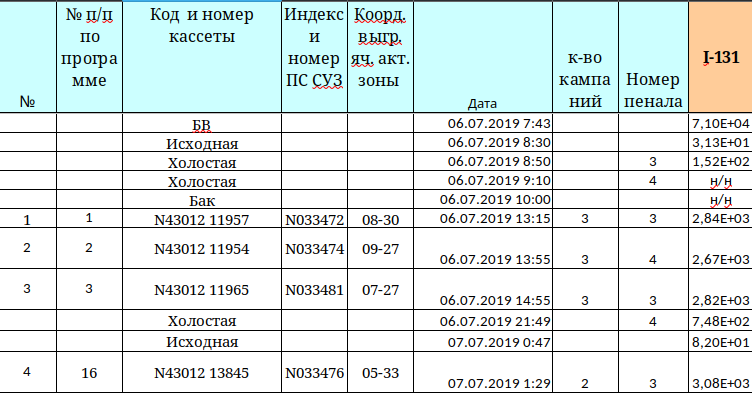
\includegraphics[width=1\linewidth]{pics/ris4} % изображения хранятся в подкаталоге pics
	\caption{Пример входных данных}
	\label{fig:ris4} % эта метка позволяет ссылаться на рисунок в тексте
\end{figure}

\begin{figure}[H]
	\centering
	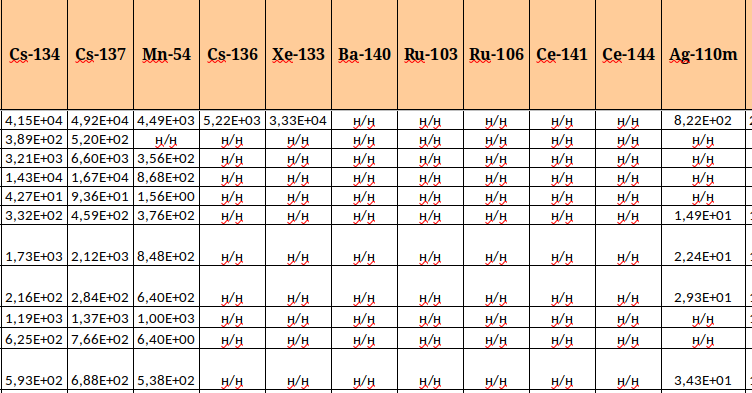
\includegraphics[width=1\linewidth]{pics/ris5} % изображения хранятся в подкаталоге pics
	\caption{Пример входных данных}
	\label{fig:ris5} % эта метка позволяет ссылаться на рисунок в тексте
\end{figure}

Как видно из примера, входные данные содержат строки и столбцы, которые используются в других расчётах. Следовательно, для использования в приложении эти данные необходимо очистить. 

Чтение файла из табличных файлов(таких как .xls, .xlsx, .ods) реализовано в методе read\_excel() библиотеки pandas. Данная функция возвращает объект DataFrame, который передаётся в метод очистки под определённый шаблон входных данных. Фрагмент реализация метода, отвечающего за очистку DataFrame представлена на листинге~\ref{lst:1}. 

\begin{flushleft}
\needspace{3\baselineskip}
\captionof{Program}{Метод очистки данных} \label{lst:1}
\begin{MyCodes}
def _clear_data(self, df):
	# На текущий момент данные очищаются под конкретный шаблон пробных данных.
	# Делаем срез DataFrame, используем первые 14 столбцов
	df = df.iloc[:,0:14] 
	# Переименовываем столбцы для удобного анализа
	df.rename(columns = {
		"№":"Id1",
		"№ п/п по программе":"Id2",
		"Код  и номер кассеты":"Name",
		"Индекс и номер ПС СУЗ":"Index",
		"Коорд. выгр. яч. акт. зоны ":"Coordinates",
		"Дата":"DateTime",
		"к-во кампаний":"Age",
		"Номер пенала":"IdPenal"}, inplace = True)
	
	for i in range(0, len(df.columns.to_list())):
		column = df.columns.to_list()[i]
		df.replace({column:"-"}, np.NaN, inplace=True) # Заменяем спец. символы
		df.replace({column:"н/н"}, np.NaN, inplace=True)
	
	# Заполняем пропуски и приводим типы
	df["Age"]=df["Age"].fillna(0.0).astype(int)
	df["IdPenal"]=df["IdPenal"].fillna(0.0).astype(int)
	df["Id2"]=df["Id2"].fillna(0.0).astype(int)
	
	...
	
	return penals, penals_id, cassetes

\end{MyCodes}
\end{flushleft}

\subsection{Анализ данных}

\subsubsection{Поиск выбросов}

Поиск выбросов в разрабатываемом приложении реализован в качестве метода у сущности, представляющей выборку. Метод основан на вычислении критического значения для выборки по заданному критерию. После вычисления критического значения объект DataFrame агрегируется по условию. Полученные строки удаляются из исходного DataFramе и производится повторный расчёт критического значения согласно параграфу~\ref{povtor}. 

Фрагмент реализации метода поиска выбросов, связанный с расчётом критических значений представлен в листинге~\ref{lst:check}. Полная реализация данного метода представлена в приложении~\ref{check}.

\begin{flushleft}
\needspace{3\baselineskip}
\captionof{Program}{Фрагмент метода поиска выбросов} \label{lst:check}
\begin{MyCodes}
...

# method_type - аргумент функции, указывающих метод поиска выбросов
if method_type=="IQR":
	# Расчёт параметров для метода "IQR"
	a_q1 = df[criteriums[i]].quantile(q=.25)
	a_q3 = df[criteriums[i]].quantile(q=.75)
	a_IQR = a_q3-a_q1
	
	a_corosion_q1 = df[criteriums[i]].quantile(q=.25)
	a_corosion_q3 = df[criteriums[i]].quantile(q=.75)
	a_corosion_IQR = a_corosion_q3-a_corosion_q1
	
	a_crit = (a_q3+1.7*a_IQR) # Критическое значение для реперных ПД
	a_corosion_crit = (a_corosion_q3+1.7*a_corosion_IQR) # Критическое значение ПК
else:
	# Расчёт параметров для метода "3 сигм"
	a_mean = df[criteriums[i]].mean()
	a_corosion_mean = df["Mn-54"].mean()
	a_std = df[criteriums[i]].std()
	a_corosion_std = df["Mn-54"].std() # Критическое значение для реперных ПД
	a_crit = self.crit_value(a_mean, a_std, len(df))
	a_corosion_crit = self.crit_value(a_corosion_mean,
		a_corosion_std, len(df)) # Критическое значение для ПК

# Аггрегируем DataFrame по критическому значению
# В результате получаем таблицу ТВС, 
# у которых аномально высокие активности реперных ПД
crit_df = df[(df[criteriums[i]]>a_crit)].reset_index(drop=True)

# Для ТВС, полученных в crit_df
# проверяется выброс по продуктам коррозии
non_hermetic = crit_df[crit_df["Mn-54"]<a_corosion_crit]
recheck = crit_df[crit_df["Mn-54"]>=a_corosion_crit]

...
\end{MyCodes}
\end{flushleft}

Кроме того, в приведённом листинге для вычисления критического значения по методу "3 сигм" используется метод crit\_value, который имеет довольно простую реализацию:

\begin{flushleft}
\needspace{3\baselineskip}
\captionof{Program}{Функция вычисления критического значения, для } \label{lst:сrit_value}
\begin{MyCodes}
	
def crit_value(self, mean, std, n):
	student = {2:12.7, 3:4.3, 4:3.18, 5:2.78, 6:2.57, 7:2.45, 8:2.36, 9:2.31, 10:2.26}
	
	# Исключаем mean==np.NaN и std==np.Nan
	if (not pd.notna(mean)) or (not pd.notna(std)): return 0
	
	# Возвращаем пороговое значение, выше которого считать выбросом
	return mean+student.get(n,3)*std
	
\end{MyCodes}
\end{flushleft}

В данной реализации используются значения критерия Стьюдента из таблицы~\ref{tab:Student}.

Результатом выполнения метода, представленного в листинге~\ref{lst:check}, являются 3 таблицы:

\begin{itemize}
	\item Таблица негерметичных ТВС, содержит исходные данные о ТВС, а так же радионуклиды, на основании которых предполагается негерметичность.
	\item Таблицы ТВС для повторной проверки, содержит исходные данные о ТВС, а так же радионуклиды, на основании которых предполагается негерметичность.
	\item Таблица расчётных параметров, содержащая информацию о математическом ожидании, среднеквадратическом отклонении, а так же о квантилях.
\end{itemize}

\subsubsection{Статистические тесты}

Все статистические тесты, описанные в 2.2.2-2.2.4, реализованы в библиотеке scipy.stats, что довольно сильно упрощает реализацию данного модуля. Основной задачей во время разработки данного модуля являлось определение достаточного количества повторений тестов(Манна-Уитни и Крамера-Уэлча) согласно алгоритму, предложенному в 2.2.3. Увеличение количества повторений существенно замедляет работу модуля, но в то же время малое число повторений не обеспечивает требуемой точности. 

На основе модельных данных, я проводил тесты для 3 выборок и сравнивал длины доверительных интервалов для N от 10 до 1000 повторений. По результатам исследования было установлено, что:
\begin{itemize}
 \item при изменении числа повторений с 10 до 100, длина доверительного интервала при уровне значимости $\alpha = 0,05$ длина доверительного интервала изменяется в среднем на $\approx 0,2-0,3$ и составляет $\approx 0,05$. Время выполнения метода при этом в среднем изменяется на 0,4 секунды
 
 \item при изменении числа повторений от 100 до 1000, длина доверительного интервала при уровне значимости $\alpha = 0,05$ длина доверительного интервала изменяется в среднем на $\approx 0,02-0,03$ и составляет $\approx 0,018$. Время выполнения метода при этом в среднем изменяется на 2,1-2,5 секунды.
 
\end{itemize}

В результате данного испытания я пришёл к выводу, что длина доверительного интервала $\approx 0,05$ является приемлемой, поэтому выбрал количество повторений N=100. Реализация теста по критерию Манна-Уитни представлена в листинге \ref{lst:mann-whitney}.

\begin{flushleft}
	\needspace{3\baselineskip}
	\captionof{Program}{Реализация теста Манна-Уитни} \label{lst:mann-whitney}
	\begin{MyCodes}
def mannwhitney_test(self, criterium):
	pvalues = []
	
	for i in range(0,100):
		n1, n2 = random_generate(self.df, criterium)
		
		statistic, pvalue = stats.mannwhitneyu(n1, n2, alternative='two-sided')
		
		pvalues.append(pvalue)
	
	pvalues = pd.Series(pvalues)
	pvalue = pd.Series(pvalues).mean()
	confidence = stats.norm.interval(confidence=0.95, loc=np.mean(pvalues),
		scale=stats.sem(pvalues))
	
	return (format(confidence[0], '.3f'), format(confidence[1], '.3f'))
	
	\end{MyCodes}
\end{flushleft}


\subsection{Пользовательский интерфейс}

Данный раздел содержит описание инструментов и трудностей, с которыми я столкнулся во время разработки приложения, а также примеры реализаций графических элементов, используемых в моём приложении.

\subsubsection{Основные окна приложения}

На основании анализа пользовательского сценария использования, представленного в \ref{Scenarii}, был сделан вывод, что проектируемое приложение будет состоять 4 окон(2 основных и 2 диалоговых):

\begin{itemize}
	\item Диалоговое окно импорта файла
	\item Окно анализа пеналов
	\item Окно анализа выборок
	\item Диалоговое окно с результатами статистических тестов 
\end{itemize}

Хочу отметить, что разделение окна анализа выборок и окна анализа пеналов сделано намеренно, т.к. при переходе в окно анализа выборок должна сохраняться не только возможность выбрать выборки заново без изменения в логике. Кроме того подразумевается, что работа по пеналам может проводиться параллельно, следовательно, именно поэтому окно анализа выборок было решено сделать самостоятельным окном, а не интегрировать внутрь другого.

\subsubsection{Окно импорта файла}

При открытии файла используется класс QFileDialog, который предоставляет окно выбора файла. Удобство этого класса заключается в том, что имеется возможность установить фильтры на расширения файлов, чтобы не вызывать исключений при попытке открыть файл с расширением, которое не поддерживается. Пример окна для выбора фала представлен на рисунке~\ref{fig:ris7}.

\begin{figure}[H]
	\centering
	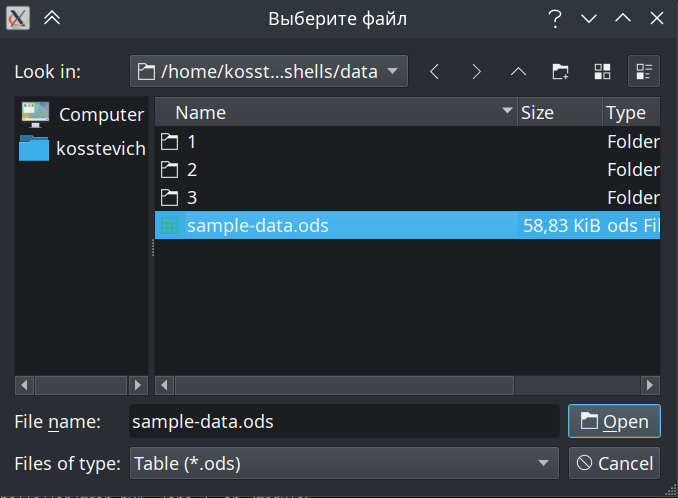
\includegraphics[width=1\linewidth]{pics/ris7} % изображения хранятся в подкаталоге pics
	\caption{Окно выбора файла}
	\label{fig:ris7} % эта метка позволяет ссылаться на рисунок в тексте
\end{figure}

\subsubsection{Интеграция Matplotlib в качестве QWidget}

Во время разработки приложения я столкнулся с трудностью интеграции графиков Matplotlib в QWidjet. Проблема заключалась в том, что базовый класс Matplotlib создаёт для графиков независимые окна. Данная реализация мне не подходит, т.к. разрабатываемое приложение должно иметь целостный формат.

Изучив документацию библиотеки, я нашёл класс FigureCanvasQTAgg, предоставляющий backend-реализацию холста Canvas для PyQt. На основе него был разработан собственный пользовательский виджет для использования в моём приложении. Реализация пользовательского виджета представлена в листинге~\ref{lst:canvas}

\begin{flushleft}
\needspace{3\baselineskip}
\captionof{Program}{Пользовательский класс, интегрирующий Сanvas в QWidget} \label{lst:canvas}
\begin{MyCodes}
class PlotData(FigureCanvasQTAgg): 
	# Виджет для отрисовки графиков, использующий matplotlib
	def __init__(self, parent=None):
		sns.set(style="whitegrid", context="paper")
		self.fig = plt.figure(figsize=(15, 10))
		self.axes = self.fig.add_subplot(111)
		super(PlotData, self).__init__(self.fig)
	
	def draw_plot(self, df, axe_x="Id1",
			axe_y="I-131", type = "barplot", name=None):
		self.axes.cla()
		# Метод позволяет рисовать разные виды графиков seaborn
		# Выбор типа графика происходит по аргументу type
		getattr(sns,type)(data=df, x=axe_x, y=axe_y, ax=self.axes)
		plt.title(label= name, fontsize=16)
\end{MyCodes}
\end{flushleft}

Кроме реализации холста я использовал класс NavigationToolbar2QT, который предоставляет возможности навигации, редактирования легенды, а также экспорт графика в формате изображения. На рисунке~\ref{fig:ris8} красной рамкой выделены реализованные мною классы.

\begin{figure}[H]
	\centering
	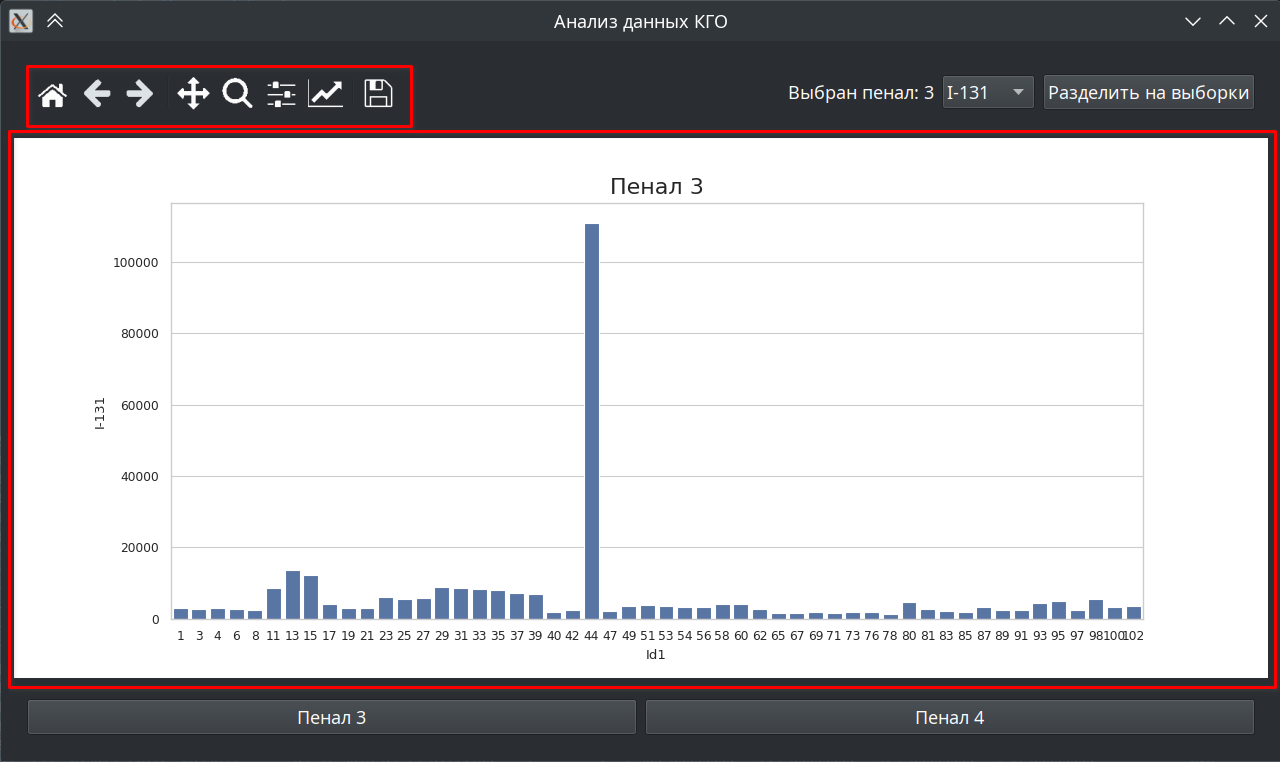
\includegraphics[width=1\linewidth]{pics/ris8} % изображения хранятся в подкаталоге pics
	\caption{Главное окно приложения}
	\label{fig:ris8} % эта метка позволяет ссылаться на рисунок в тексте
\end{figure}

\subsubsection{Главное окно приложения}

Пример внешнего вида главного окна приложения приведён на рисунке \ref{fig:ris8}. Данное окно реализовано с использованием элементов Qt:

\begin{itemize}
	\item QPushButton --- класс, отвечающий за кнопку.
	\item QLabel --- класс, позволяющий выводить текстовую информацию.
	\item QComboBox --- класс, реализующий выпадающий список.
	\item QHBoxLayout --- класс, позволяющий располагать виджеты в горизонтальной разметке
	\item QVBoxLayout --- класс, позволяющий располагать виджеты в вертикальной разметке
\end{itemize}

Кнопки, отвечающие за переход по пеналам, реализованы динамически в зависимости от количества пеналов в исходных данных.

\subsubsection{Окно анализа выборок}

Пример реализации окна анализа выборок представлен на рисунке~\ref{fig:ris10}.

\begin{figure}[H]
	\centering
	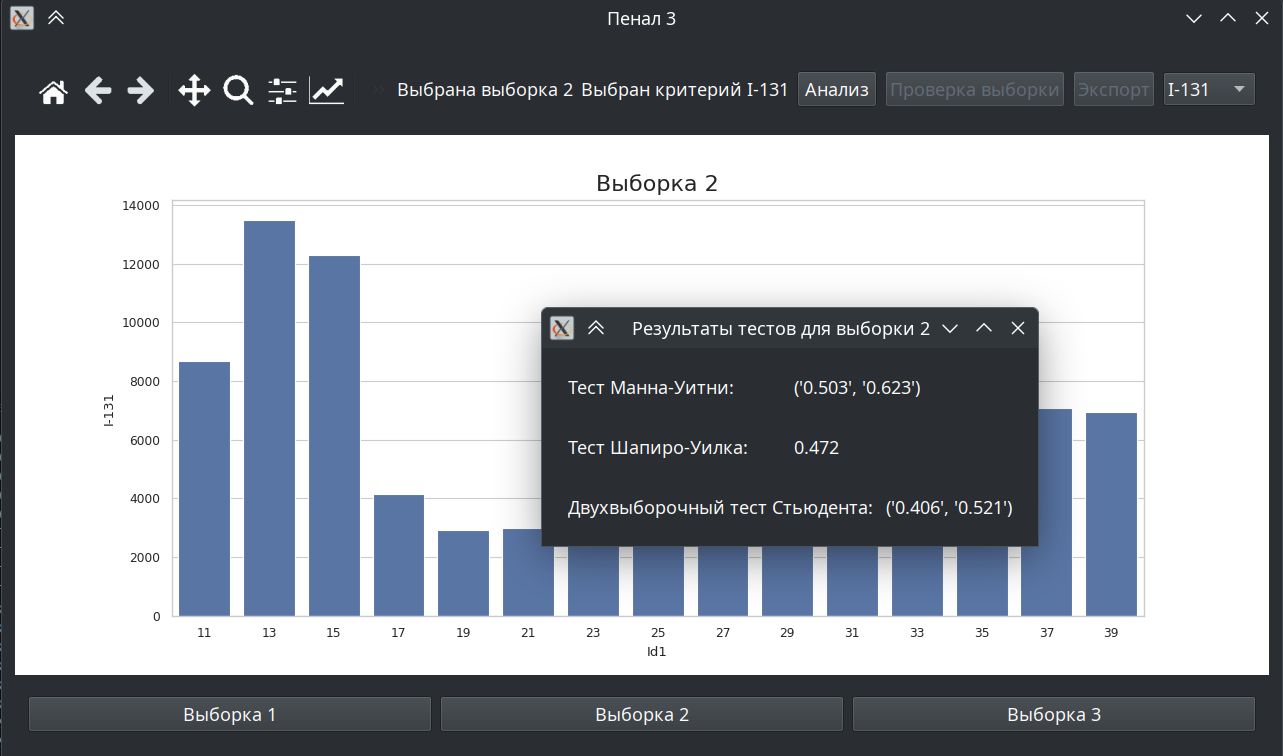
\includegraphics[width=1\linewidth]{pics/ris10} % изображения хранятся в подкаталоге pics
	\caption{Окно анализа выборок}
	\label{fig:ris10} % эта метка позволяет ссылаться на рисунок в тексте
\end{figure}

Несмотря на схожесть с окном анализа выборок, данное окно имеет более сложную структуру. В частности, класс PlotData, описанный в 4.4.3, после проведения поиска выбросов заменяется на класс QTableWidget, который содержит выходную информацию в табличном виде. Данный функционал реализован с применением класса QStackedWidget, который позволяет отображать только один из нескольких дочерних объектов. Пример табличного вывода представлен на рисунке~\ref{fig:ris14}.

\begin{figure}[H]
	\centering
	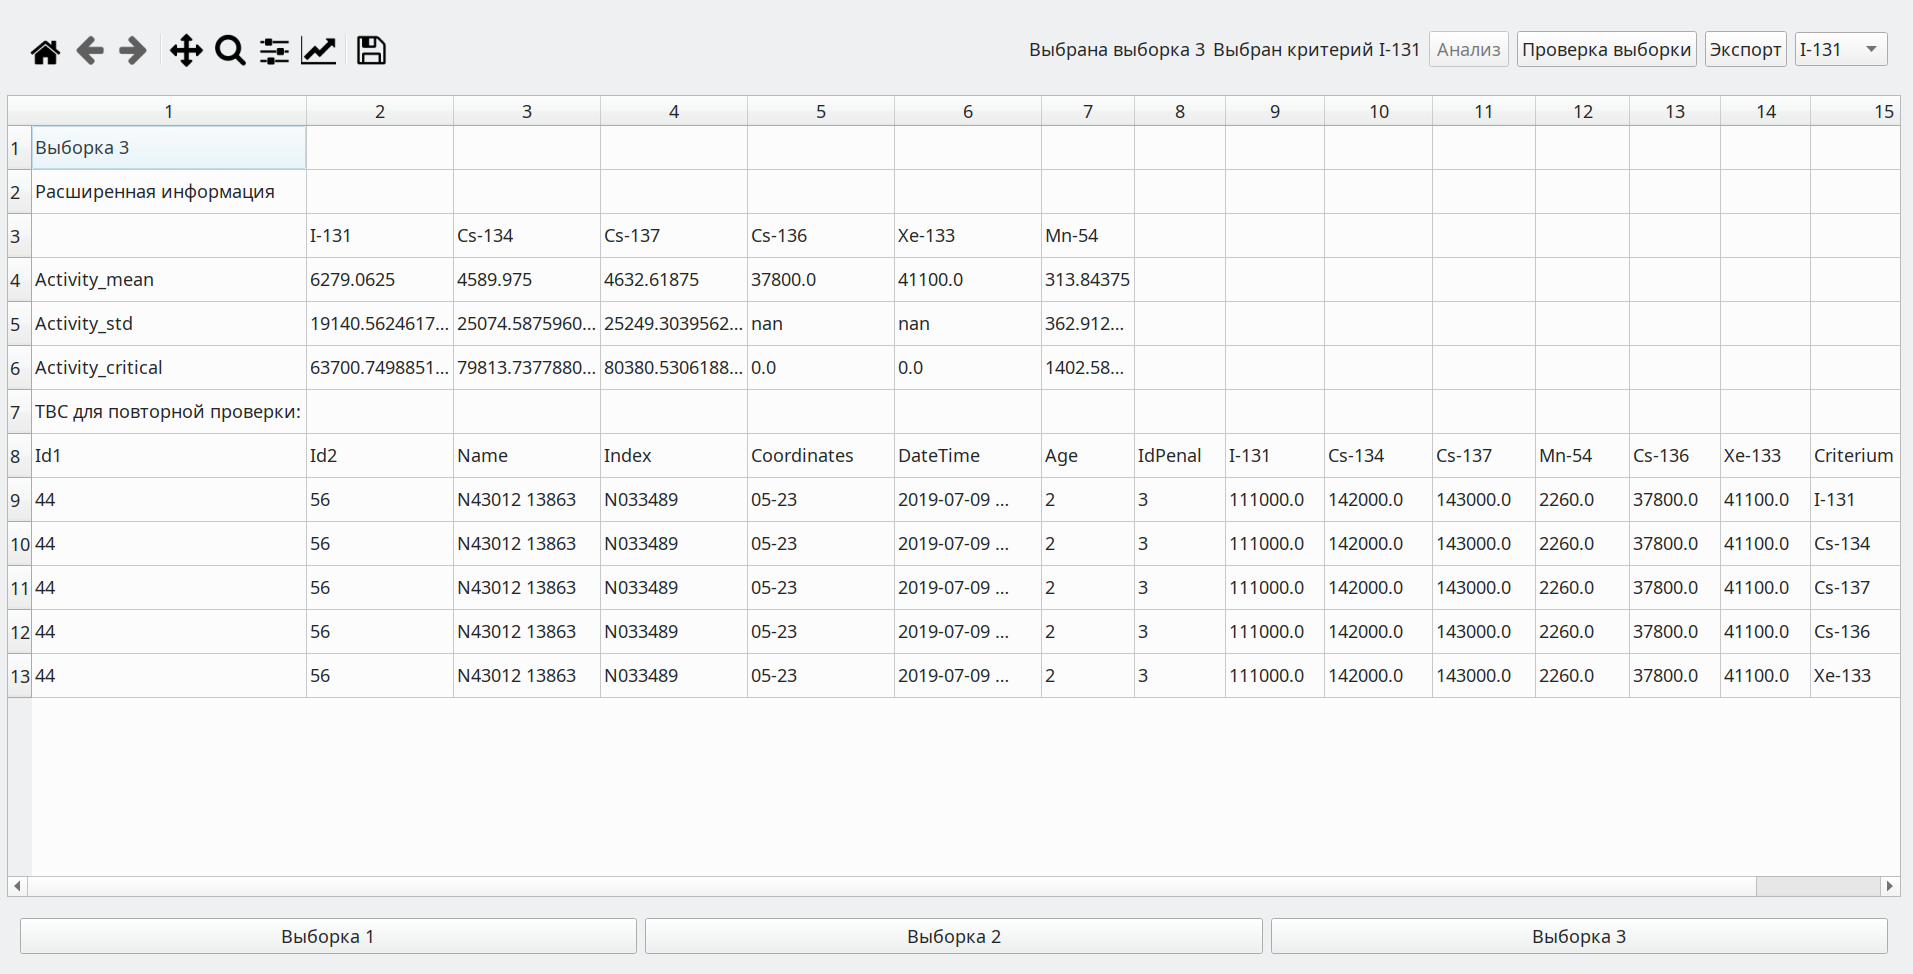
\includegraphics[width=1\linewidth]{pics/ris14} % изображения хранятся в подкаталоге pics
	\caption{Представление табличной информации через QTableWidget}
	\label{fig:ris14} % эта метка позволяет ссылаться на рисунок в тексте
\end{figure}

После проведения необходимого анализа, имеется возможность экспорта таблицы в .ods формат. Пример экспортированного файла приведён на рисунке~\ref{fig:ris12}.

\begin{figure}[H]
	\centering
	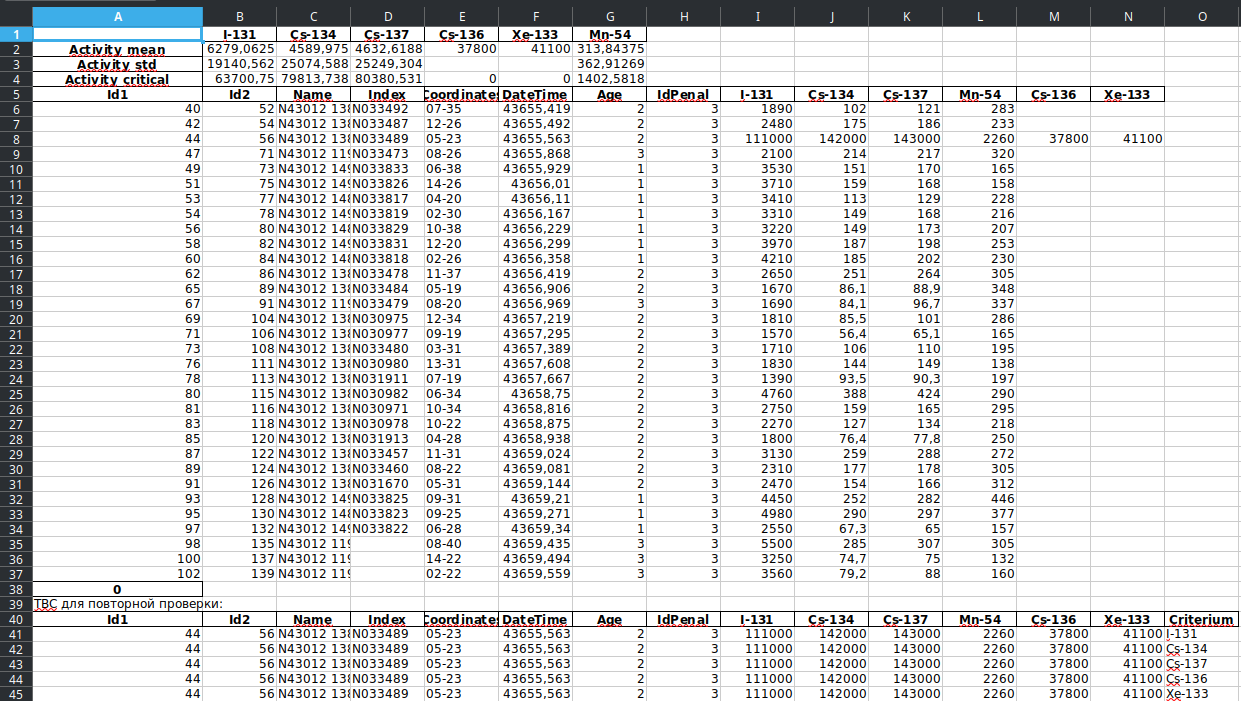
\includegraphics[width=1\linewidth]{pics/ris12} % изображения хранятся в подкаталоге pics
	\caption{Пример выходного файла}
	\label{fig:ris12} % эта метка позволяет ссылаться на рисунок в тексте
\end{figure}

%Интеграция графиков Matplotlib в QtWidget